\section{Merge Sort}
\label{sec:merge-sort-teo}

Desenvolvido por \href{https://en.wikipedia.org/wiki/John_von_Neumann}{Jon Von Neumann} em 1945, o \textit{Merge Sort} é um algoritmo de \href{https://en.wikipedia.org/wiki/Divide-and-conquer_algorithm}{dividir para conquistar}, que subdivide uma lista em singletons e os mescla em sublistas ordenadas até que exista apenas uma sublista, esta sublista é a lista original ordenada. Imagine o seguinte caso:

Você tem um baralho de cartas e gostaria de organizá-lo, seguindo o conceito do \textit{Merge Sort} você trabalha da seguinte forma:
\begin{itemize}
	\item \textbf{Divisão:} Primeiro você divide o baralho em dois baralhos menores. Cada um desses baralhos é dividido novamente até que cada sub-baralho tenha uma carta.
	\item \textbf{"Merge" (Mescla):} Nesse momento, com cada sub-baralho com uma carta, todos estão ordenados, então você começa a juntar os sub-baralhos comparando duas cartas de cada baralho e colocando-as em ordem crescente. Assim dois grupos de uma carta se tornam um baralho de duas cartas ordenadas. Em seguida, dois baralhos de duas cartas são mesclados para formar um baralho de quatro cartas, e assim por diante, até que todas as cartas estejam combinadas novamente, mas agora ordenadas.
\end{itemize}
\begin{figure}[!ht]
	\centering
	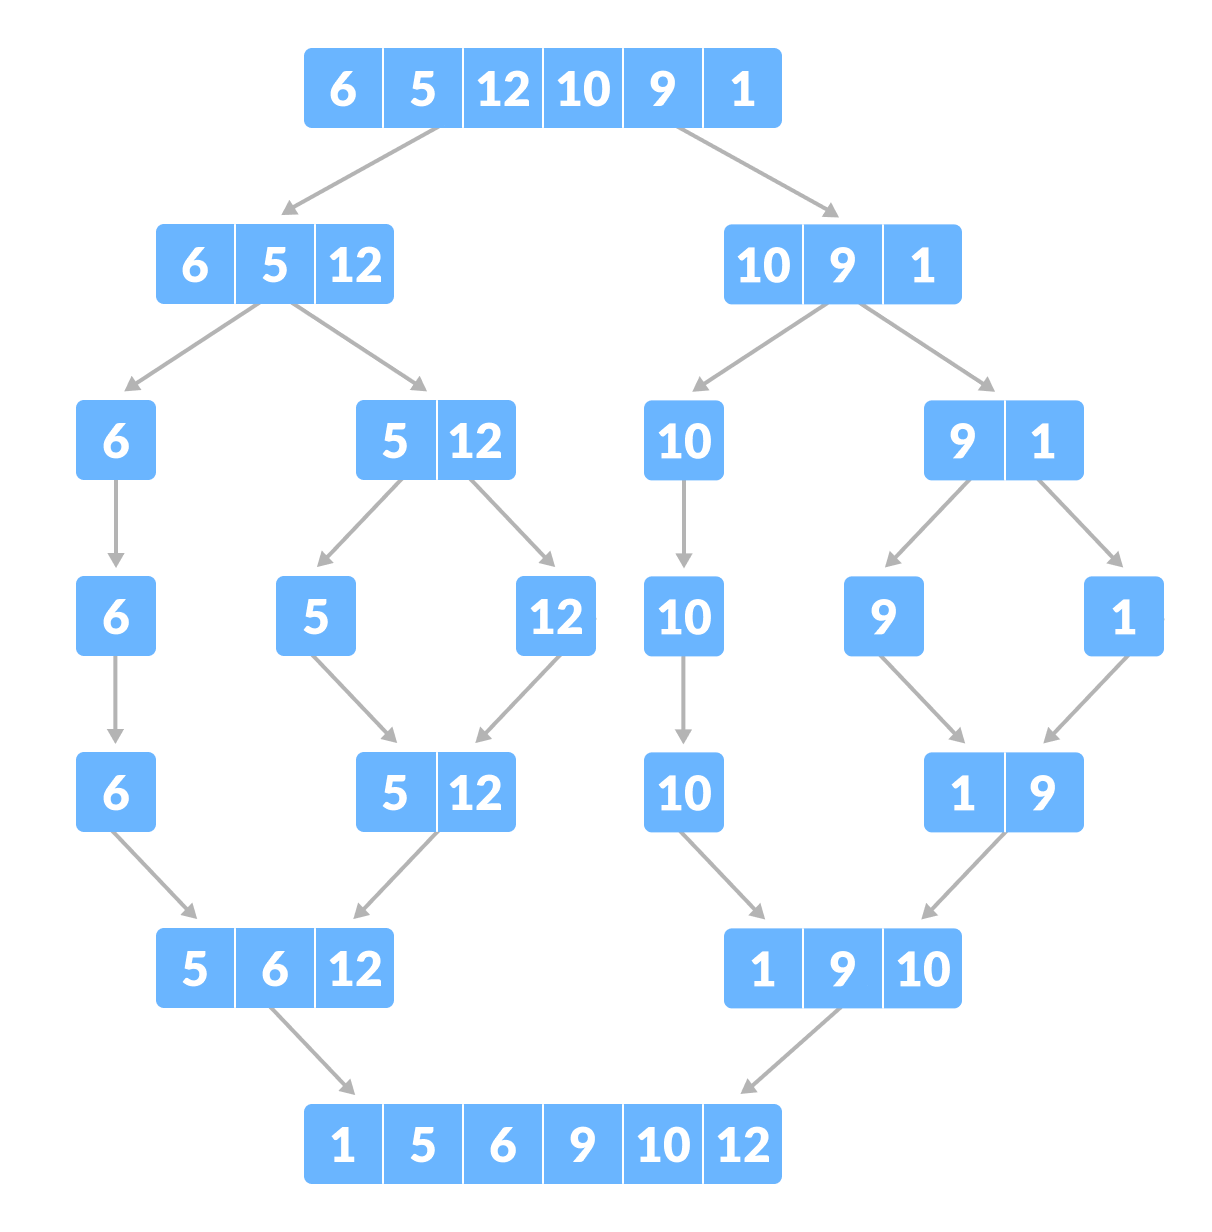
\includegraphics[scale=0.4]{figures/merge-sort-example_0.png}
	\caption{Diagrama exemplo de um Merge Sort}
	\label{fig:merge_sort_example_0}
\end{figure}

\FloatBarrier

\newpage

\subsection{Merge Sort Recursivo}

Dito isso, agora fica mais fácil estabelecer o pseudocódigo na forma recursiva. O caso base será se a lista tem no máximo elemento, pois já está ordenada. No caso recursivo, pelo teorema da recursão temos acesso ao "caso anterior", ou seja a primeira metade e segunda metade da lista original ordenadas, portanto, podemos mesclá-las.

\begin{algorithm}
	\label{algo:merge_sort_pseudo}
	\begin{algorithmic}[1]
		\Require{$\mathbf{lista}  = x_0, x_1, \ldots, x_{N-1}$}
		\Function{MergeSort}{$\mathbf{lista}$}
		\If{tamanho da \textbf{lista} $\leq 1$} \Return
		\EndIf
		\State \Return {Merge(MergeSort($1^a$ metade da \textbf{lista}), MergeSort($2^a$ metade da \textbf{lista})}
		\EndFunction
	\end{algorithmic}
\end{algorithm}

\FloatBarrier

\subsection{Merge Sort Iterativo}

\textbf{TODO}

\subsection{Função auxiliar Merge}

\noindent
Nos resta agora apenas definir a função \textbf{Merge}, que vai ser responsável por mesclar duas listas que estão ordenadas. Para tal, a função deve comparar um elemento da primeira lista com um da segunda e anexar o menor elemento entre os dois no final da lista resultado. Por exemplo:

\begin{figure}[!ht]
	\centering
	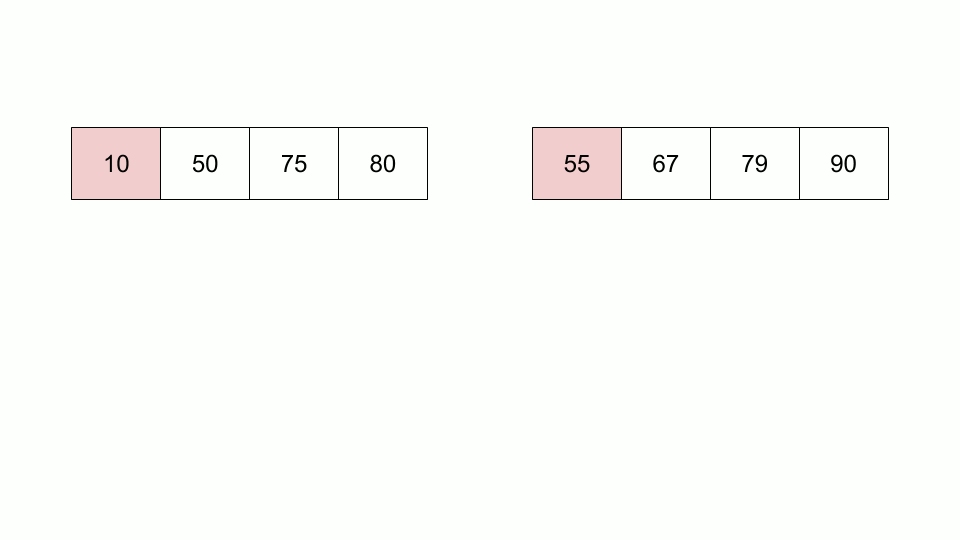
\includegraphics[scale=0.3]{figures/merge/merge-function-1.png}
	\caption{Comparando o primeiro elemento da primeira lista com o primeiro da segunda}
\end{figure}
\begin{figure}[!ht]
	\centering
	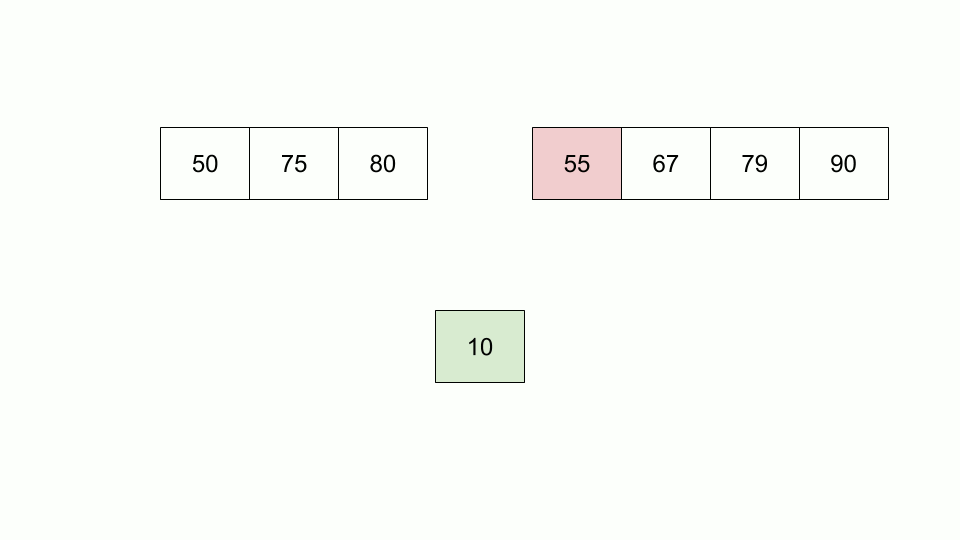
\includegraphics[scale=0.3]{figures/merge/merge-function-3.png}
	\caption{10 é menor que 55, então é anexado no final da lista resultado}
\end{figure}
\begin{figure}[!ht]
	\centering
	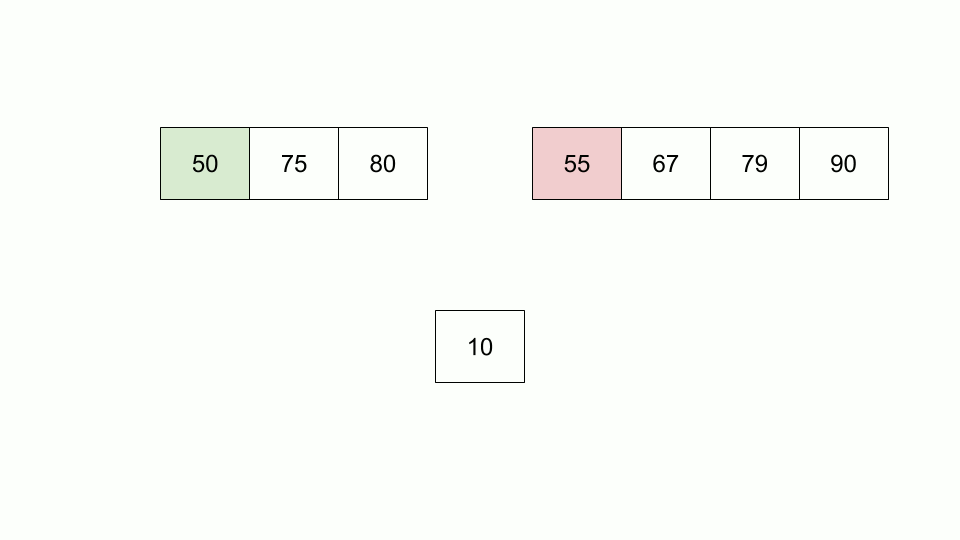
\includegraphics[scale=0.3]{figures/merge/merge-function-5.png}
	\caption{Comparando o próximo elemento da primeira lista}
\end{figure}
\begin{figure}[!ht]
	\centering
	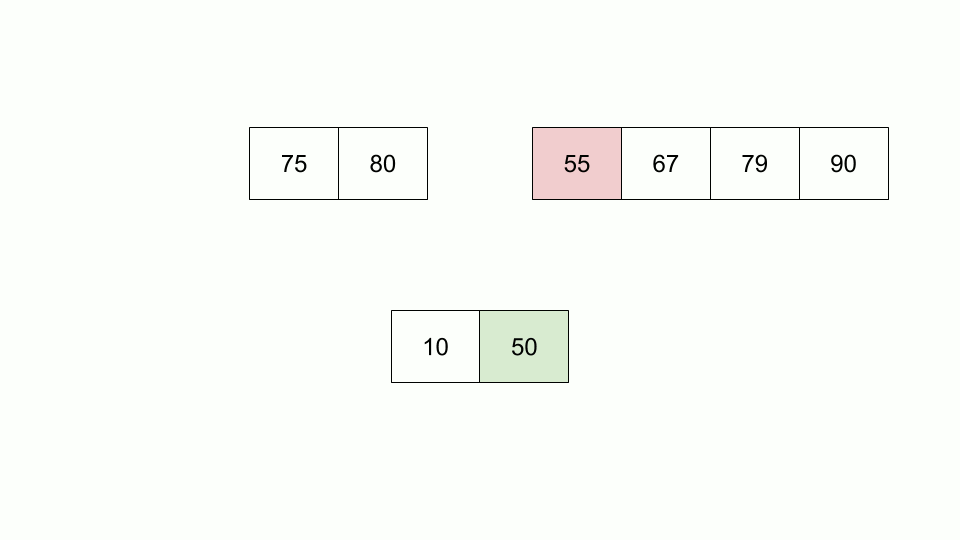
\includegraphics[scale=0.3]{figures/merge/merge-function-6.png}
	\caption{50 é menor que 55, então é anexado no final da lista resultado}
\end{figure}
\begin{figure}[!ht]
	\centering
	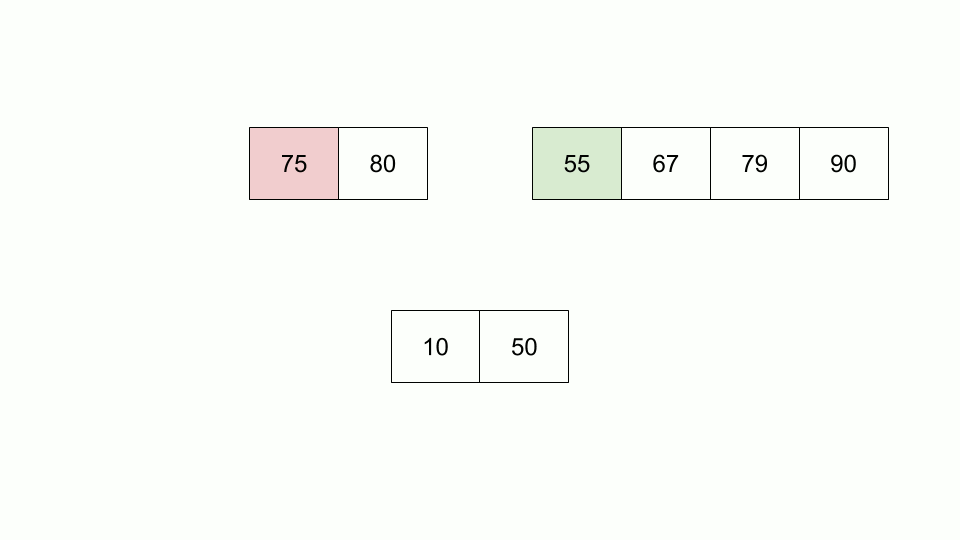
\includegraphics[scale=0.3]{figures/merge/merge-function-8.png}
	\caption{Comparando o próximo elemento da primeira lista}
\end{figure}
\begin{figure}[!ht]
	\centering
	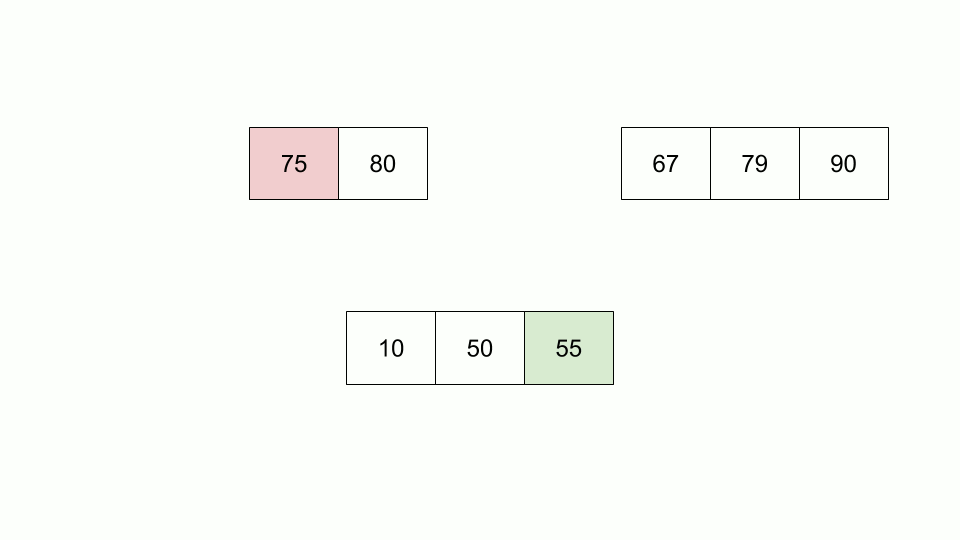
\includegraphics[scale=0.3]{figures/merge/merge-function-9.png}
	\caption{55 é menor, então é anexado no final da lista resultado}
\end{figure}
\begin{figure}[!ht]
	\centering
	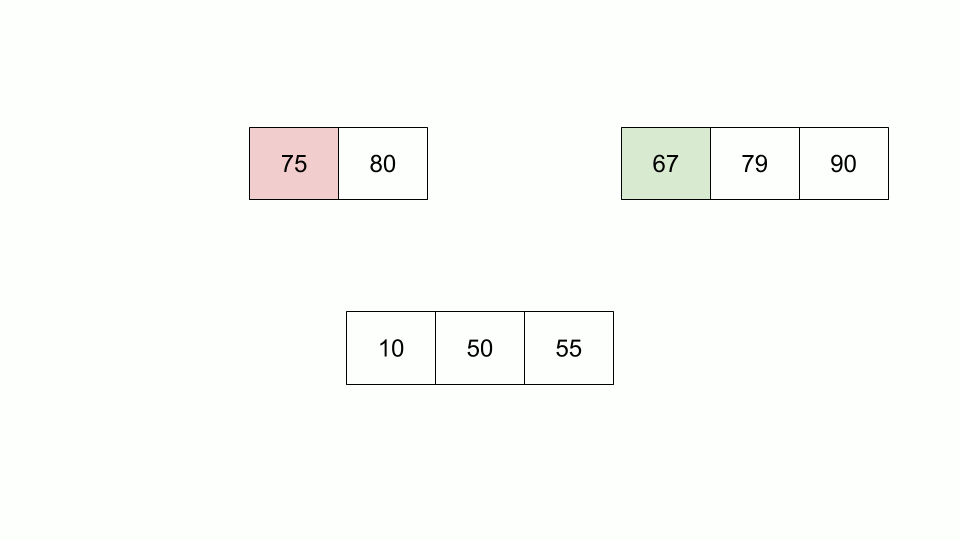
\includegraphics[scale=0.3]{figures/merge/merge-function-11.png}
	\caption{Comparando o próximo elemento da segunda lista}
\end{figure}

\FloatBarrier

E o algoritmo vai continuar até que a lista resultado esteja completa com os elementos da primeira e segunda lista.

Dito isso, construímos o pseudocódigo dessa função da seguinte forma:

\begin{algorithm}
	\label{algo:merge_aux_pseudo}
	\begin{algorithmic}[1]
		\Require{$\mathbf{listaEsquerda} = x_0, x_1, \ldots, x_{N - 1}$, $\mathbf{listaDireita} = y_0, y_1, \ldots, y_{M - 1}$}
		\Ensure{A \textbf{listaResultado} ordenada com os elementos da \textbf{listaEsquerda} e \textbf{listaDireita}}
		\Statex
		\Function{Merge}{$\mathbf{listaEsquerda}$, $\mathbf{listaDireita}$}
		\State $E, D, R = 0$ \Comment Esses serão os indexadores de cada lista
		\State $\mathbf{listaResultado} = 0, 0,\ldots, 0$
		\While{$E < N$ e $D < M$}
		\If{\textbf{listaEsquerda}(E) < \textbf{listaDireita}(D)}
		\State $\mathbf{listaResultado}(R).push(\mathbf{listaDireita}(D)$)
		\State $E = E + 1$ \Comment Partimos para o próximo elemento
		\Else
		\State $\mathbf{listaResultado}(R).push(\mathbf{listaEsquerda}(D)$)
		\State $D = D + 1$
		\EndIf
		\State $R = R + 1$
		\EndWhile
		\State $\rhd \text{ Como uma das listas vai esgotar primeiro que a outra, copiamos os elementos}$
		\State $\text{restantes para a }\mathbf{listaResultado}$
		\While {\textbf{listaEsquerda} ou \textbf{listaDireita} tiver elementos}
		\State adicione os elementos na \textbf{listaResultado}
		\EndWhile
		\State \Return \textbf{listaResultado}
		\EndFunction
	\end{algorithmic}
\end{algorithm}

\subsection{Análise de complexidade}

Para analisar qual é a complexidade de tempo da \textbf{Merge sort}, nas suas duas versões, vamos estabelecer primeiro qual é a complexidade da função \textbf{Merge}. A partir do \href{algo:merge_aux_pseudo}{pseudocódigo} da função, é facil de ver que durante sua execução ela sempre vai percorrer o tamanho máximo entre a \textbf{listaEsquerda} e \textbf{listaDireita}, portanto, sua complexidade na notação de complexidade assintótica é $O(n)$, $\Theta(n)$ e $\Omega(n)$.

\subsubsection{Análise da versão iterativa}

\textbf{TODO}

\subsubsection{Análise da versão recursiva}

Analisando o corpo da função, teremos dois casos: caso o tamanho da lista ($n$) seja menor ou igual 1 e caso contrário.

\begin{algorithm}
	\begin{algorithmic}[0]
		\If{tamanho da \textbf{lista} $\leq 1$} \Return
		\EndIf
		\State \Return {Merge(MergeSort($1^a$ metade da \textbf{lista}), MergeSort($2^a$ metade da \textbf{lista})}
	\end{algorithmic}
\end{algorithm}
\FloatBarrier

No primeiro caso, é facil de ver que a complexidade da função para uma lista de qualquer tamanho é constante, ou seja, $O(1)$, $\Theta(1)$ e $\Omega(1)$. Caso contrário, observa-se que a função chama a si mesmo duas vezes, uma para cada metade da lista. Ademais, a função \textit{Merge}, com complexidade linear para qualquer entrada, é chamada em cada etapa recursiva. Portanto, estabelecemos a relação de recorrência da \textit{Merge sort} recursiva como:

\begin{align*}
	\label{recc:rec_merge_sort}
	T(n) =
	\begin{cases}
		O(1),                   & \text{se $n \leq 1$}  \\
		2T(\frac{n}{2}) + O(n), & \text{caso contrário}
	\end{cases}
\end{align*}

Uma vez estabelecida a relação de recorrência, vamos usar primeiro a \textbf{Árvore de recorrência} como método. Comecemos estabelecendo seu diagrama:

\[\begin{tikzcd}[sep=small]
		&&&& {T(n)} \\
		\\
		&& {T(\frac{n}{2})} &&&& {T(\frac{n}{2})} \\
		& {T(\frac{n}{4})} & {T(\frac{n}{4})} &&&& {T(\frac{n}{4})} & {T(\frac{n}{4})} \\
		{T(\frac{n}{8})} & {T(\frac{n}{8})} & {T(\frac{n}{8})} & {T(\frac{n}{8})} && {T(\frac{n}{8})} & {T(\frac{n}{8})} & {T(\frac{n}{8})} & {T(\frac{n}{8})} \\
		\vdots & \vdots & \vdots & \vdots & \vdots & \vdots & \vdots & \vdots & \vdots
		\arrow[from=1-5, to=3-3]
		\arrow[from=1-5, to=3-7]
		\arrow[from=3-3, to=4-2]
		\arrow[from=3-3, to=4-3]
		\arrow[from=3-7, to=4-7]
		\arrow[from=3-7, to=4-8]
		\arrow[from=4-2, to=5-1]
		\arrow[from=4-2, to=5-2]
		\arrow[from=4-3, to=5-3]
		\arrow[from=4-3, to=5-4]
		\arrow[from=4-7, to=5-6]
		\arrow[from=4-7, to=5-7]
		\arrow[from=4-8, to=5-8]
		\arrow[from=4-8, to=5-9]
	\end{tikzcd}\]
\FloatBarrier

Uma vez estabelecida a árvore de recorrência, podemos tabular o tamanho da entrada, seu custo por nó e quantidade de nós para cada nível da árvore:


\begin{table}[h!]
	\centering
	\begin{tabular}{lrrr}
		\toprule
		Nível da árvore & Tamanho da entrada & Custo por nó    & Quantidade de nós \\
		\midrule
		0               & $n$                & n               & $1 = 2^0$         \\
		1               & $\frac{n}{2^1}$    & $\frac{n}{2^1}$ & $2 = 2^1$         \\
		2               & $\frac{n}{2^2}$    & $\frac{n}{2^2}$ & $4 = 2^2$         \\
		3               & $\frac{n}{2^3}$    & $\frac{n}{2^3}$ & $8 = 2^3$         \\
		$\vdots$        & $\vdots$           & \vdots          & \vdots            \\
		i               & $\frac{n}{2^i}$    & $\frac{n}{2^i}$ & $2^i$             \\
		\bottomrule
	\end{tabular}
\end{table}
\FloatBarrier

Em seguida, para estabelecer o somatório que calcula a complexidade da função, precisamos identificar o valor de $i$ para quando $T(\frac{n}{2^i}) = T(1)$, assim, teremos:

\begin{align*}
	\frac{n}{2^i} = 1 & \Longrightarrow n = 2^i      \\
	                  & \Longrightarrow \log_2 n = i
\end{align*}

Dessa forma, a complexidade da função para $\Omega$, $\Theta$ e $O$ será dada pelo resultado do somatório:

\begin{align*}
	\sum_{i = 0}^{\log_2 n} \frac{n}{2^i} \cdot 2^i & = \sum_{i = 0}^{\log_2 n}n  \\
	                                                & = n\sum_{i = 0}^{\log_2 n}1 \\
	                                                & = n \cdot \log_2 n
\end{align*}


Pelo método do \textbf{Teorema mestre}, o mesmo resultado ocorre em ainda menos etapas. Pelo teorema, temos que estabelecendo a relação de recorrência nessa forma:

$$
	T(n) = aT\left(\frac{n}{b}\right) + \Theta\left(n^{k}\right)
$$

Para algum $a \geq 1$, $b \geq 1$, e $k \geq 0$. Vale que:

\begin{enumerate}
	\item Se $a \geq b^k$, então $T(n)$ é $\Theta(n^{\log_b a})$.
	\item Se $a = b^k$, então $T(n)$ é $\Theta(n^k \cdot \log_b a)$.
	\item Se $a < b^k$, então $T(n)$ é $\Theta(n^k)$.
\end{enumerate}

A partir da \href{recc:rec_merge_sort}{relação de recorrência estabelecida}, tome $a = 2$, $b = 2$ e $k = 1$. Como $b^k = 2 = a$, logo, $T(n) = \Theta(n \cdot \log_2 n)$. Como foi estabelecido que o pior caso, o melhor e caso médio iam ter a mesma complexidade, logo, a \textit{Merge sort} também tem as complexidades $O(n \cdot \log_2 n)$ e $\Omega(n \cdot \log_2 n)$.

%  TODO:
% - Análise de complexidade
